\documentclass{article}
\usepackage{caption}
\usepackage{amssymb}
\usepackage{array}
\usepackage{geometry}
\usepackage{scrextend}
\usepackage{amsmath}
\usepackage{hyperref}
\usepackage{graphicx}
\usepackage{pdfpages}
\usepackage{multicol}

\title{EE102 Homework 2}
\author{Jacob Guenther}

\geometry{
	a4paper,
	total={170mm,257mm},
	left=20mm,
	top=20mm,
}

\newcommand{\problemstatement}[3]{
\noindent
\begin{tabular}{ m{0.5cm} m{42em} m{0.5cm} }
	({#1}) & {#2} & {#3}pts
\end{tabular}
}

\begin{document}

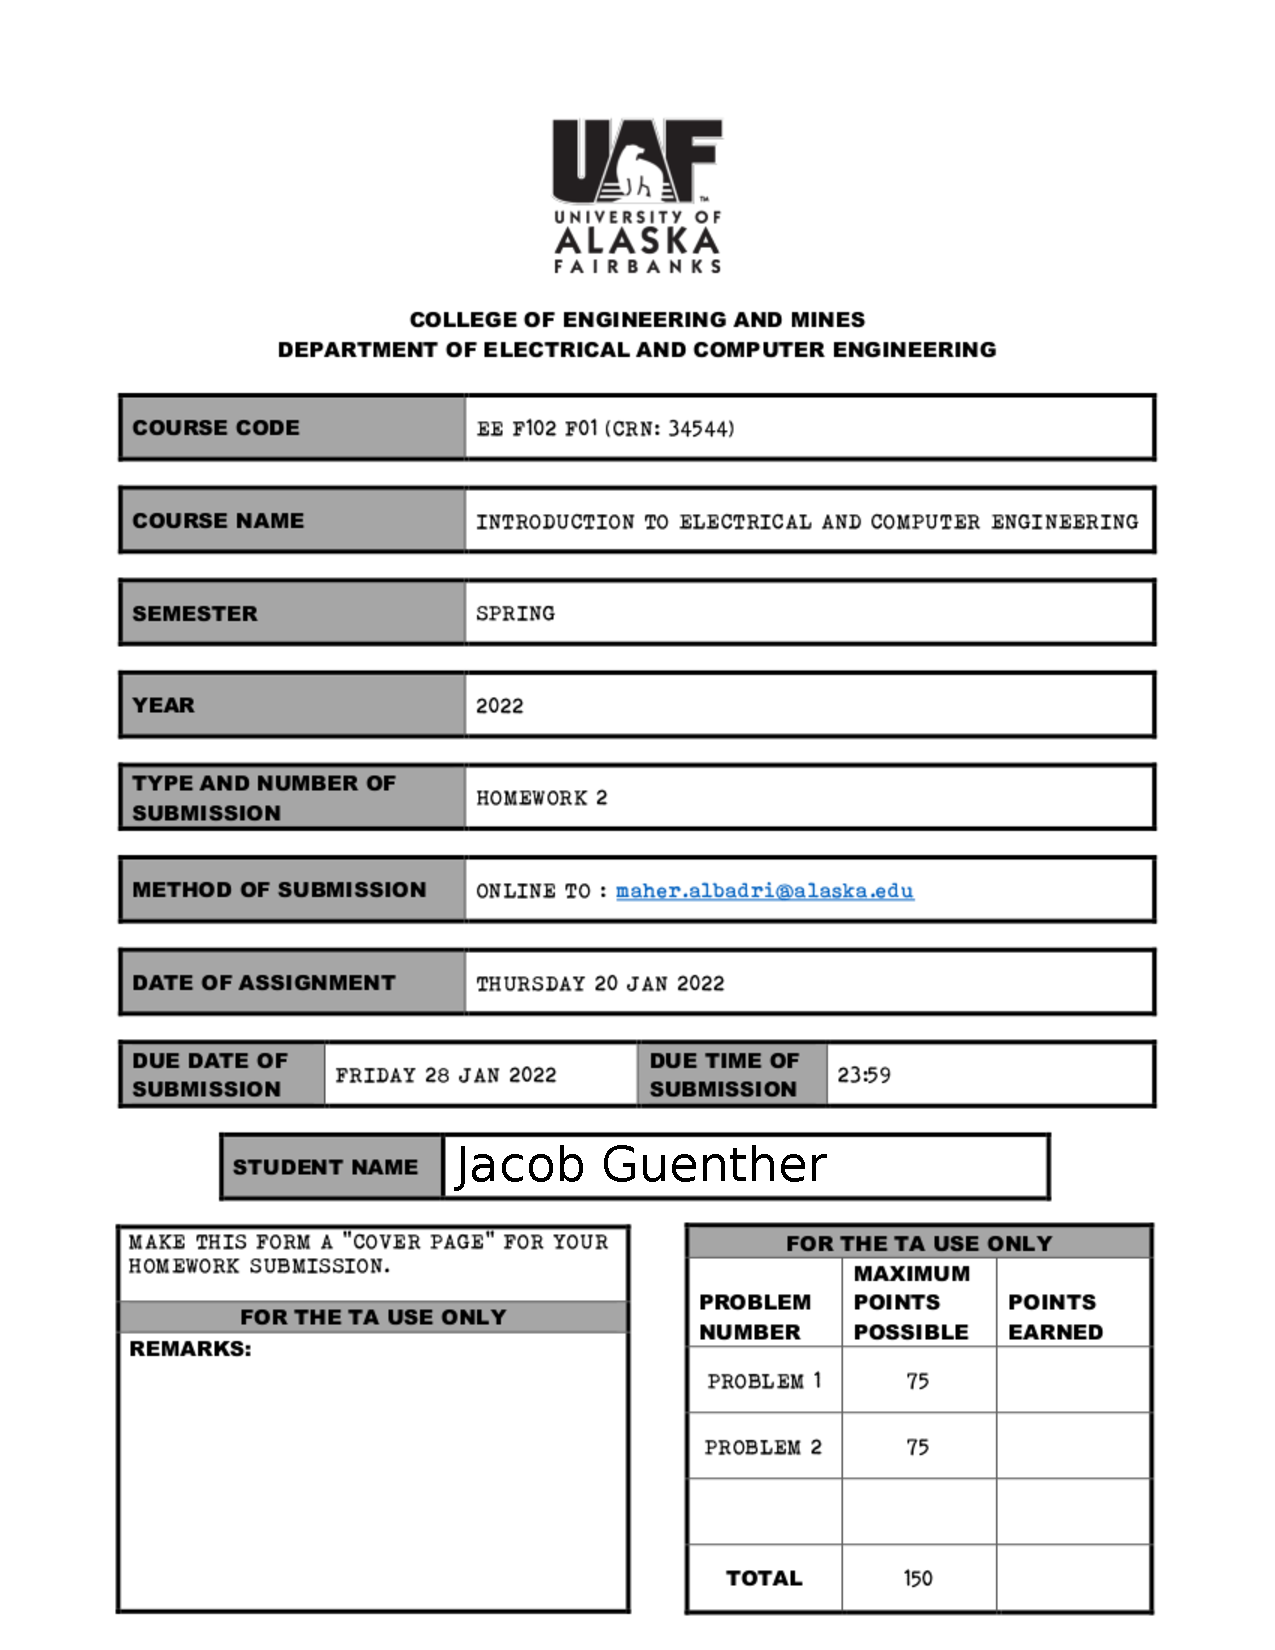
\includepdf[pages=1,pagecommand={}]{HW2cover.pdf}

\section{Problem HW-1-1}
\problemstatement{a}{For the current signal shown, determine:}{25}
\begin{itemize}
	\item The DC offset "A", in amperes
	\item The amplitude "B", in amperes
	\item The period "T", in seconds
	\item The frequency "f", in hertz
	\item The angular frequency "$\omega$", in rad/s
	\item The phase shift angle "$\Phi$", in degrees
\end{itemize}
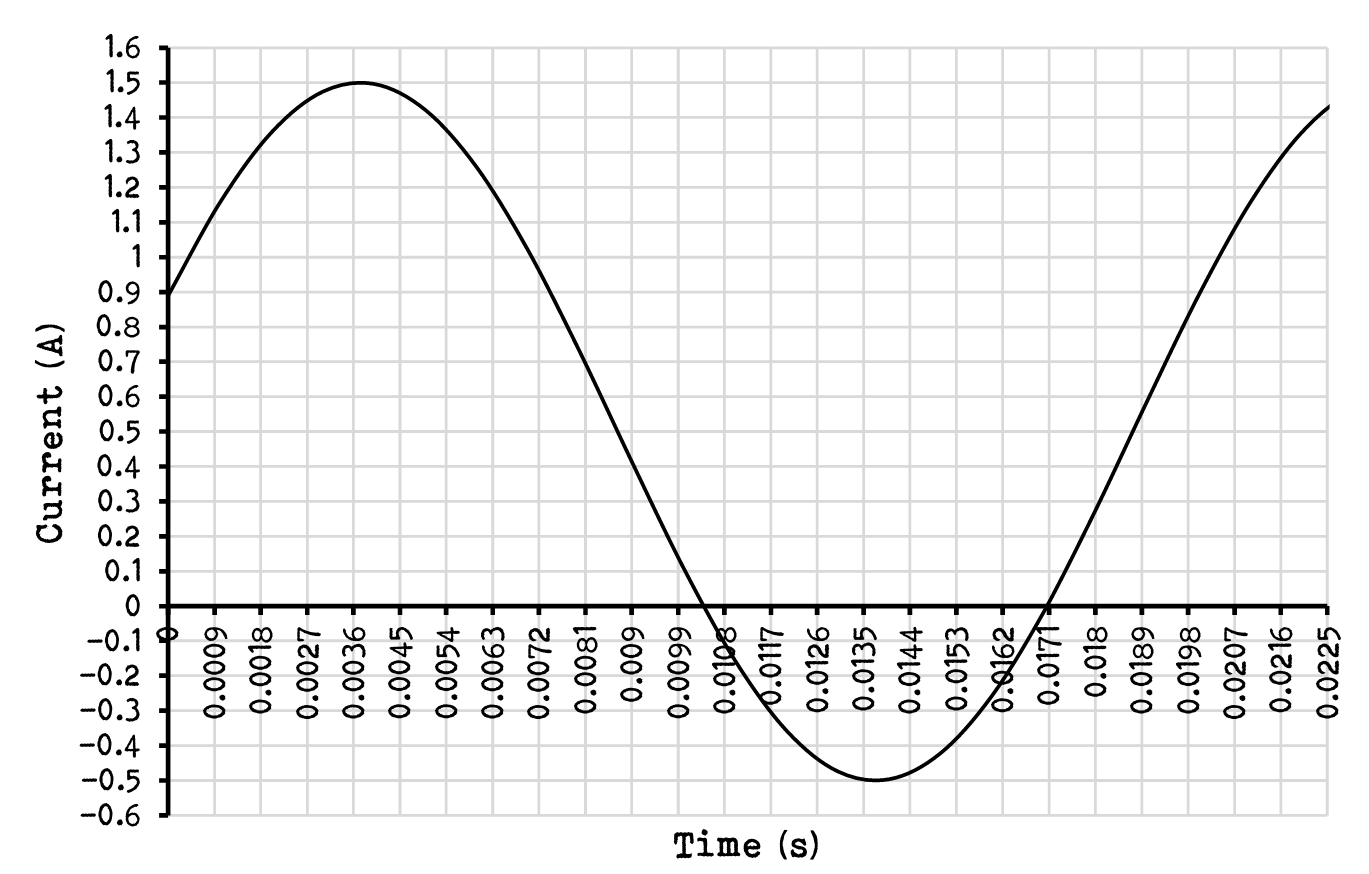
\includegraphics[width=\textwidth]{figure_hw2_1}
\begin{equation}
	i(t)= \text{A} + \text{B} sin( \omega t + \Phi )
\end{equation}
\begin{addmargin}[1.5cm]{0em}
	\noindent
	\textbf{Note:} \\
	\begin{equation}
		2\text{B} = I_{max} - I_{min}
	\end{equation}	
	\begin{equation}
		\text{A} = {I_{max} + I_{min} \over 2}
	\end{equation}
	\begin{equation}
		\text{T} = t_2 - t_1
	\end{equation}
	\begin{equation}
		f = {1 \over \text{T}}
	\end{equation}
	\begin{equation}
		\omega = {2 \pi \over \text{T}}
	\end{equation}
		\[ I_{max} = 1.5 \text{A} \]
		\[ I_{min} = -0.5 \text{A} \]
		\[ t_1 = 0 \text{s} \]
		\[ t_2 = 0.0198 \text{s} \]
		\[ i(0) = 0.9 \text{A} \]
	\noindent
	\textbf{Solution:} \\
	\begin{align*}
		\text{A} &= {1.5 \text{A} + (-0.5) \text{A} \over 2} \\
		&= 0.5 \text{A} \\
		2\text{B} &= 1.5 \text{A} - (-0.5) \text{A} \\
		\text{B} &= {1.5 \text{A} - (-0.5) \text{A} \over 2} \\
		&= 1 \text{A} \\
		\text{T} &= 0.0198 \text{s} - 0 \text{s} \\
		&= 0.0198 \text{s} \\
		f &= {1 \over 0.0198 s} \\
		&= 50.5 \text{Hz} \\
		\omega &= {2 \pi \over 0.0198s} \\
		&= 317.33 \text{rad/s} \\
		0.9 \text{A} &= 0.5 \text{A} + 1.0 \text{A} sin(317.33 \text{rad/s} \cdot 0 \text{s} + \Phi) \\
		0.9 \text{A} - 0.5 \text{A} &= 1.0 \text{A} sin(\Phi) \\
		{0.4 \text{A} \over 1.0 \text{A}} &= sin(\Phi) \\
		\Phi &= sin^{-1}(0.4) \\
		&= 0.4115 \text{rad}
	\end{align*}
	\noindent
	\textbf{Answer:}
	\begin{itemize}
		\item The DC offset A is \textbf{0.5 A}
		\item The amplitude B is \textbf{1 A}
		\item The period T is \textbf{0.0198 s}
		\item The frequency is \textbf{50.5 Hz}
		\item The angular frequency is \textbf{317.33 rad/s}
		\item The phase shift is \textbf{0.4115 rad}
	\end{itemize}
\end{addmargin}

\newpage
\problemstatement{b}{1200 C charge moves uniformly through a conductor for 10 minutes. Calculate the current, in amperes, passing through the conductor.}{25}
\begin{addmargin}[1.5cm]{0em}
	\noindent
	\textbf{Note:} \\
	\begin{equation}
		I = {\Delta Q \over \Delta t}
	\end{equation}
	\begin{equation}
		1 \text{min} = 60 \text{s}
	\end{equation}
	\noindent
	\textbf{Solution:} \\
	\begin{align*}
		t &= 10 \text{min} \cdot {60 \text{s} \over 1 \text{min}} \\
		&= 600 \text{s} \\
		I &= {1200 \text{C} \over 600 \text{s}} \\
		&= 2 \text{A}
	\end{align*}
	\noindent
	\textbf{Answer:} The current passing through the conductor is \textbf{2 A}.
\end{addmargin}

\newpage
\problemstatement{c}{A uniform current of 3.5 A flows in a circuit for 30 minutes. Calculate the total charge passed through any point in the circuit.}{25}
\begin{addmargin}[1.5cm]{0em}
	\noindent
	\textbf{Solution:} \\
	\begin{align*}
		t &= 30 \text{min} \cdot {60 \text{s} \over 1 \text{min}} \\
		&= 1800 \text{s} \\
		\text{Q} &= 3.5 \text{A} \cdot 1800 \text{s} \\
		&= 6300 \text{C}
	\end{align*}
	\noindent
	\textbf{Answer:} The total charge passing through the circuit is \textbf{6.3 kC}.
\end{addmargin}

\newpage
\section{Problem HW-1-2}
\problemstatement{a}{A neutral body has $10^{10}$ electrons added to it. Then, a negative charge of 0.1 $\mu$C was removed from the body. Calculate the body’s final charge, in $\mu$C.}{25}
\begin{addmargin}[1.5cm]{0em}
	\noindent
	\textbf{Note:} \\
	\begin{equation}
	\text{electron charge} = -1.602177 \times 10^{-19} \text{C}
	\end{equation}
	\begin{equation}
	1 \text{C} = 1 \times 10^6 \mu \text{C} 
	\end{equation}
	\begin{align*}
		Q_i &= 0 \text{C}
	\end{align*}
	\noindent
	\textbf{Solution:} \\
	\begin{align*}
		Q_e &= (1 \times 10^{10})(-1.602177 \times 10^{-19} \text{C}) \\
		&= -1.602177 \times 10^{-9} \text{C} \cdot { 10^6 \mu \text{C} \over 1 \text{C} } \\
		&= -0.001602177 \mu C \\
		Q_c &= -(-0.1 \mu C) \\
		&= 0.1 \mu C \\
		Q_f &= Q_i + Q_e + Q_c \\
		&= 0 \mu \text{C} + -0.001602177 \mu C + 0.1 \mu C \\
		&= 0.098397823 \mu \text{C} \\
		&= 0.098 \mu \text{C}
	\end{align*}
	\noindent
	\textbf{Answer:} The body's final charge is \textbf{0.098 $\mu$C}
\end{addmargin}

\newpage
\problemstatement{b}{A battery rated at 60 Ah supplies 1.0 mA to a resistive load. Determine the battery life in hours.}{25}
\begin{addmargin}[1.5cm]{0em}
	\noindent
	\textbf{Note:} \\
	\begin{equation}
	\text{life[h]} = {\text{capacity[Ah]} \over \text{drain[A]}}
	\end{equation}
	\begin{equation}
	1 \text{A} = 1000 \text{mA}
	\end{equation}
	\noindent
	\textbf{Solution:} \\
	\begin{align*}
		\text{drain} &= 1.0 \text{mA} \cdot { 1 \text{A} \over 1000 \text{mA} } \\
		&= 0.001 \text{A} \\
		\text{life} &= {60 \text{Ah} \over 0.001 \text{A} } \\
		&= 60000 \text{h}
	\end{align*}
	\noindent
	\textbf{Answer:} The battery's life is \textbf{60000 h} \\
\end{addmargin}

\newpage
\problemstatement{c}{Electric potential of 120 V is established when energy is utilized to move $10^{20}$ electrons from point A to point B. Calculate the value of the energy, in kJ, used to do the work.}{25}
\begin{addmargin}[1.5cm]{0em}
	\noindent
	\textbf{Note:} \\
	\begin{equation}
		E=V \cdot Q
	\end{equation}
	\noindent
	\textbf{Solution:} \\
	\begin{align*}
		Q &= 10^{20} \cdot 1.602177 \times 10^{-19}  \text{C} \\
		&= 16.02177  \text{C} \\
		E &= 120  \text{V} 16.02177  \text{C} \\
		&= 1922.6124  \text{J} \\
		&= 1.9226124  \text{kJ} \\
		&= 1.9  \text{kJ} \\
	\end{align*}
	\noindent
	\textbf{Answer:} The energy used to move the electrons between points A and B is \textbf{1.9 kJ} \\
\end{addmargin}

\newpage
\section{References}
[1] Denise Thorsen, Maher Al-Badri, INTRODUCTION TO ELECTRICAL AND COMPUTER ENGINEERING, University of Alaska Fairbanks, 2022.

\end{document}